% Information-flow direction under Bottom-Up, Top-Down, and MinT reconciliation
% Panels stacked vertically, scaled down proportionally using scale and transform shape.
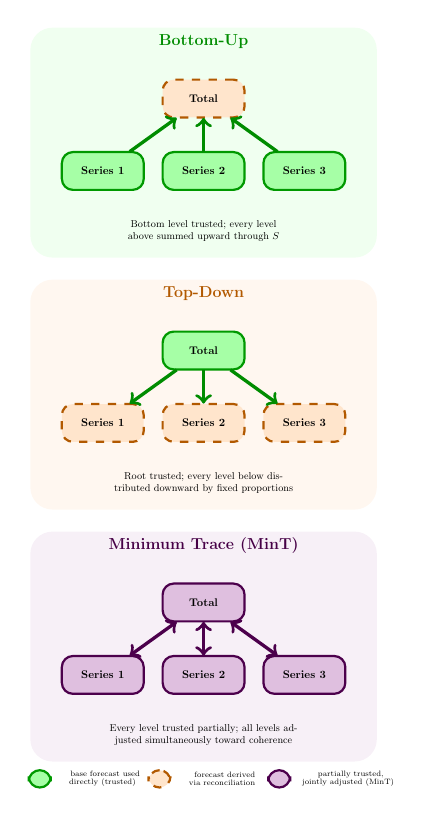
\begin{tikzpicture}[
	scale=0.4,
	every node/.style={transform shape},
	node distance   = 1.4cm and 1cm,
	topstage/.style   = {rectangle, rounded corners, thick, minimum width=2.6cm,
		minimum height=1.2cm, align=center, font=\normalsize\bfseries},
	leafstage/.style  = {rectangle, rounded corners, thick, minimum width=2.6cm,
		minimum height=1.2cm, align=center, font=\normalsize\bfseries},
	trusted/.style    = {fill=green!35, draw=green!60!black},
	derived/.style    = {fill=orange!20, draw=orange!70!black, dashed},
	minttrust/.style  = {fill=violet!25, draw=violet!60!black},
	title/.style      = {font=\Large\bfseries},
	detail/.style     = {align=center, font=\small, text width=9.5cm},
	legendbox/.style  = {rectangle, rounded corners, thick, minimum width=0.7cm, minimum height=0.55cm},
	panelbg/.style    = {rectangle, rounded corners=8pt, draw=none, minimum width=11cm, minimum height=7.3cm}
	]
	
	% ===================== Panel 1: Bottom-Up =====================
	\begin{scope}[yshift=0cm]
		\node[panelbg, fill=green!6] at (0,0.9) {};
		\node[title, color=green!55!black] (t1) at (0, 4.1) {Bottom-Up};
		
		\node[topstage, derived]  (tot1) at (0, 2.3)   {Total};
		\node[leafstage, trusted] (b1a)  at (-3.2, 0) {Series 1};
		\node[leafstage, trusted] (b1b)  at (0, 0)    {Series 2};
		\node[leafstage, trusted] (b1c)  at (3.2, 0)  {Series 3};
		
		\draw[->, very thick, green!55!black] (b1a) -- (tot1);
		\draw[->, very thick, green!55!black] (b1b) -- (tot1);
		\draw[->, very thick, green!55!black] (b1c) -- (tot1);
		
		\node[detail] at (0, -1.9) {Bottom level trusted; every level above summed upward through $S$};
	\end{scope}
	
	% ===================== Panel 2: Top-Down =====================
	\begin{scope}[yshift=-8cm]
		\node[panelbg, fill=orange!6] at (0,0.9) {};
		\node[title, color=orange!70!black] (t2) at (0, 4.1) {Top-Down};
		
		\node[topstage, trusted]  (tot2) at (0, 2.3)   {Total};
		\node[leafstage, derived] (b2a)  at (-3.2, 0) {Series 1};
		\node[leafstage, derived] (b2b)  at (0, 0)    {Series 2};
		\node[leafstage, derived] (b2c)  at (3.2, 0)  {Series 3};
		
		\draw[->, very thick, green!55!black] (tot2) -- (b2a);
		\draw[->, very thick, green!55!black] (tot2) -- (b2b);
		\draw[->, very thick, green!55!black] (tot2) -- (b2c);
		
		\node[detail] at (0, -1.9) {Root trusted; every level below distributed downward by fixed proportions};
	\end{scope}
	
	% ===================== Panel 3: MinT =====================
	\begin{scope}[yshift=-16cm]
		\node[panelbg, fill=violet!6] at (0,0.9) {};
		\node[title, color=violet!55!black] (t3) at (0, 4.1) {Minimum Trace (MinT)};
		
		\node[topstage, minttrust]  (tot3) at (0, 2.3)   {Total};
		\node[leafstage, minttrust] (b3a)  at (-3.2, 0) {Series 1};
		\node[leafstage, minttrust] (b3b)  at (0, 0)    {Series 2};
		\node[leafstage, minttrust] (b3c)  at (3.2, 0)  {Series 3};
		
		\draw[<->, very thick, violet!60!black] (b3a) -- (tot3);
		\draw[<->, very thick, violet!60!black] (b3b) -- (tot3);
		\draw[<->, very thick, violet!60!black] (b3c) -- (tot3);
		
		\node[detail] at (0, -1.9) {Every level trusted partially; all levels adjusted simultaneously toward coherence};
	\end{scope}
	
	% ===================== Shared legend =====================
	\begin{scope}[yshift=-19.3cm]
		\node[legendbox, trusted] (legA) at (-5.2, 0) {};
		\node[detail, text width=3cm, anchor=west, font=\scriptsize] at (legA.east) {\; base forecast used directly (trusted)};
		
		\node[legendbox, derived] (legB) at (-1.4, 0) {};
		\node[detail, text width=3cm, anchor=west, font=\scriptsize] at (legB.east) {\; forecast derived via reconciliation};
		
		\node[legendbox, minttrust] (legC) at (2.4, 0) {};
		\node[detail, text width=3.4cm, anchor=west, font=\scriptsize] at (legC.east) {\; partially trusted, jointly adjusted (MinT)};
	\end{scope}
	
\end{tikzpicture}